\documentclass{beamer}
\usepackage[utf8]{inputenc}

\usetheme{Madrid}
\usecolortheme{default}
\usepackage{amsmath,amssymb,amsfonts,amsthm}
\usepackage{txfonts}
\usepackage{tkz-euclide}
\usepackage{listings}
\usepackage{adjustbox}
\usepackage{array}
\usepackage{tabularx}
\usepackage{gvv}
\usepackage{lmodern}
\usepackage{circuitikz}
\usepackage{tikz}
\usepackage{graphicx}
\usepackage{comment} % Required for comment environment
\usepackage{gensymb} % For \degree symbol
\usepackage{mathtools} % For \coloneqq
\usepackage{xparse} % For \DeclareTCBListing
\usepackage{tcolorbox}
\tcbuselibrary{minted,breakable,xparse,skins}

\setbeamertemplate{page number in head/foot}[totalframenumber]

\definecolor{bg}{gray}{0.95}
\DeclareTCBListing{mintedbox}{O{}m!O{}}{%
breakable=true,
listing engine=minted,
listing only,
minted language=#2,
minted style=default,
minted options={%
linenos,
gobble=0,
breaklines=true,
breakafter=,,
fontsize=\small,
numbersep=8pt,
#1},
boxsep=0pt,
left skip=0pt,
right skip=0pt,
left=25pt,
right=0pt,
top=3pt,
bottom=3pt,
arc=5pt,
leftrule=0pt,
rightrule=0pt,
bottomrule=2pt,
toprule=2pt,
colback=bg,
colframe=orange!70,
enhanced,
overlay={%
\begin{tcbclipinterior}
\fill[orange!20!white] (frame.south west) rectangle ([xshift=20pt]frame.north west);
\end{tcbclipinterior}},
#3,
}
\lstset{
language=C,
basicstyle=\ttfamily\small,
keywordstyle=\color{blue},
stringstyle=\color{orange},
commentstyle=\color{green!60!black},
numbers=left,
numberstyle=\tiny\color{gray},
breaklines=true,
showstringspaces=false,
}

\title
{4.3.33}
\date{September 28, 2025}
\author
{EE25BTECH11043 - Nishid Khandagre}

\begin{document}

\frame{\titlepage}

\begin{frame}{Question}
If the coordinates of the middle point of the portion of a line intercepted between the coordinate axes is $\myvec{3\\2}$, then the equation of the line will be
\end{frame}

\begin{frame}{Theoretical Solution}
The equation of a line is
\begin{align}
\vec{n}^\top\vec{x} = c
\end{align}
Where $\vec{n} = \myvec{n_1 \\ n_2}$ is the normal vector and $\vec{x}$ is the position vector.
\end{frame}

\begin{frame}{Theoretical Solution}
X-axis intercept is at $\vec{A}$
\begin{align}
\vec{n}^\top\vec{A}=c\\
\myvec{n_1&n_2}\myvec{a\\0}=c\\
n_1a=c\\
\vec{A}=\myvec{\frac{c}{n_1}\\0}
\end{align}
\end{frame}

\begin{frame}{Theoretical Solution}
Y-axis intercept is at $\vec{B}$
\begin{align}
\vec{n}^\top\vec{B}=c\\
\myvec{n_1&n_2}\myvec{0\\b}=c\\
n_2b=c\\
\vec{B}=\myvec{0\\\frac{c}{n_2}}
\end{align}
\end{frame}
\begin{frame}{Theoretical Solution}
The $\vec{M}$ is the midpoint of $\vec{A}$ and $\vec{B}$\\
Given $\vec{M} = \myvec{3 \\ 2}$.
\begin{align}
\vec{M} &= \frac{\vec{A} + \vec{B}}{2} \\
\myvec{3\\2}&= \frac{1}{2} \myvec{\frac{c}{n_1} \\ 0} + \frac{1}{2}\myvec{0 \\ \frac{c}{n_2}}\\
\myvec{3\\2}&= \myvec{\frac{c}{2n_1} \\ \frac{c}{2n_2}}
\end{align}
\end{frame}

\begin{frame}{Theoretical Solution}
\begin{align}
\frac{c}{2n_1}&=3\\
\frac{c}{2n_2}&=2\\
\frac{n_1}{n_2} &= \frac{2}{3}
\end{align}
Let $n_1=2$ and $n_2=3$.
Then
\begin{align}
c = 6 \times 2 = 12
\end{align}

The final equation of the line is $\vec{n}^\top \vec{x} = c$
\begin{align}
\myvec{2 & 3} \vec{x} = 12
\end{align}
\end{frame}

\begin{frame}[fragile]
\frametitle{C Code}
\begin{lstlisting}
#include <stdio.h>

// Function to calculate 'a' (x-intercept) and 'b' (y-intercept)
// given the midpoint (xm, ym) of the line segment intercepted between the axes.
void findIntercepts(double xm, double ym, double *a, double *b) {
    // If the midpoint of (a, 0) and (0, b) is (xm, ym):
    // (a + 0) / 2 = xm  -> a = 2 * xm
    // (0 + b) / 2 = ym  -> b = 2 * ym
    *a = 2 * xm;
    *b = 2 * ym;
}
\end{lstlisting}
\end{frame}

\begin{frame}[fragile]
\frametitle{Python Code through shared output}
\begin{lstlisting}
import ctypes
import numpy as np
import matplotlib.pyplot as plt

# Load the shared library
lib_line = ctypes.CDLL("./code6.so")

# Define the argument types and return type for the C function
lib_line.findIntercepts.argtypes = [
    ctypes.c_double,  # xm (midpoint x-coordinate)
    ctypes.c_double,  # ym (midpoint y-coordinate)
    ctypes.POINTER(ctypes.c_double), # a (x-intercept)
    ctypes.POINTER(ctypes.c_double)  # b (y-intercept)
]
\end{lstlisting}
\end{frame}

\begin{frame}[fragile]
\frametitle{Python Code through shared output}
\begin{lstlisting}
lib_line.findIntercepts.restype = None

# Given midpoint coordinates
xm_given, ym_given = 3.0, 2.0  # Midpoint of the line segment

# Create ctypes doubles to hold the results for 'a' and 'b'
a_result = ctypes.c_double()
b_result = ctypes.c_double()

# Call the C function to find the intercepts
lib_line.findIntercepts(
    xm_given, ym_given,
    ctypes.byref(a_result),
    ctypes.byref(b_result)
)
\end{lstlisting}
\end{frame}

\begin{frame}[fragile]
\frametitle{Python Code through shared output}
\begin{lstlisting}
a_intercept = a_result.value
b_intercept = b_result.value

print(f"Given midpoint: ({xm_given:.2f}, {ym_given:.2f})")
print(f"The x-intercept (a) is: {a_intercept:.2f}")
print(f"The y-intercept (b) is: {b_intercept:.2f}")

# The equation of the line is x/a + y/b = 1
# Which can be rewritten as: b*x + a*y = a*b
# Or in standard form: b*x + a*y - a*b = 0

# For plotting, let's express y in terms of x:
# y = (-b/a) * x + b
slope = -b_intercept / a_intercept
y_intercept_calc = b_intercept
\end{lstlisting}
\end{frame}

\begin{frame}[fragile]
\frametitle{Python Code through shared output}
\begin{lstlisting}
print(f"The equation of the line is: {b_intercept:.0f}x + {a_intercept:.0f}y = {a_intercept * b_intercept:.0f}")
# Plotting the line and intercepts
plt.figure(figsize=(8, 8))

# Generate points for the line
x_vals = np.linspace(-1, 7, 400)
y_vals = slope * x_vals + y_intercept_calc
plt.plot(x_vals, y_vals, 'b-', label=f'Line: {int(b_intercept)}x + {int(a_intercept)}y = {int(a_intercept * b_intercept)}')

# Plot the x-intercept
plt.scatter(a_intercept, 0, color='red', s=100, zorder=5, label=f'X-intercept ({a_intercept:.0f}, 0)')
plt.annotate(f'({a_intercept:.0f}, 0)', (a_intercept, 0), textcoords="offset points", xytext=(5,5), ha='left')
\end{lstlisting}
\end{frame}

\begin{frame}[fragile]
\frametitle{Python Code through shared output}
\begin{lstlisting}
# Plot the y-intercept
plt.scatter(0, b_intercept, color='green', s=100, zorder=5, label=f'Y-intercept (0, {b_intercept:.0f})')
plt.annotate(f'(0, {b_intercept:.0f})', (0, b_intercept), textcoords="offset points", xytext=(5,5), ha='left')
# Plot the midpoint
plt.scatter(xm_given, ym_given, color='purple', s=100, zorder=5, label=f'Midpoint ({xm_given:.0f}, {ym_given:.0f})')
plt.annotate(f'({xm_given:.0f}, {ym_given:.0f})', (xm_given, ym_given), textcoords="offset points", xytext=(5,5), ha='left')

plt.axhline(0, color='gray', linestyle='--', linewidth=0.5)
plt.axvline(0, color='gray', linestyle='--', linewidth=0.5)
\end{lstlisting}
\end{frame}

\begin{frame}[fragile]
\frametitle{Python Code through shared output}
\begin{lstlisting}
plt.gca().set_aspect('equal', adjustable='box')
plt.xlabel('X-axis')
plt.ylabel('Y-axis')
plt.title('Equation of a Line with Given Midpoint of Intercepts')
plt.grid(True)
plt.legend()
plt.xlim(min(0, a_intercept) - 1, max(0, a_intercept) + 1)
plt.ylim(min(0, b_intercept) - 1, max(0, b_intercept) + 1)
plt.show()
# plt.savefig("fig1.png")
\end{lstlisting}
\end{frame}

\begin{frame}[fragile]
\frametitle{Python Code (Direct)}
\begin{lstlisting}
import numpy as np
import matplotlib.pyplot as plt

def line_gen_num(A, B, num_points):
    A = A.flatten()
    B = B.flatten()
    t = np.linspace(0, 1, num_points)
    points = np.outer(A, (1 - t)) + np.outer(B, t)
    return points

def plot_line_with_intercepts(mid_x, mid_y):
    # Calculate the x-intercept (a) and y-intercept (b)
    # Since (mid_x, mid_y) is the midpoint of (a, 0) and (0, b)
    # mid_x = (a + 0) / 2  => a = 2 * mid_x
    # mid_y = (0 + b) / 2  => b = 2 * mid_y
    a = 2 * mid_x
    b = 2 * mid_y
\end{lstlisting}
\end{frame}

\begin{frame}[fragile]
\frametitle{Python Code (Direct)}
\begin{lstlisting}
    # The equation of the line is x/a + y/b = 1
    # Generate points for the line
    x_intercept = np.array([a, 0]).reshape(-1, 1)
    y_intercept = np.array([0, b]).reshape(-1, 1)
    line_points = line_gen_num(x_intercept, y_intercept, 100)

    # Plotting
    plt.figure(figsize=(8, 6))
    plt.plot(line_points[0, :], line_points[1, :], "blue", label=f"Line: x/{a} + y/{b} = 1")
    # Plot the intercepts
    plt.scatter([a, 0], [0, b], color='red', s=100, zorder=5)
    plt.text(a + 0.5, 0, f'({a:.0f}, 0)', color='red')
    plt.text(0.5, b + 0.5, f'(0, {b:.0f})', color='red')
    # Plot the midpoint
    plt.scatter([mid_x], [mid_y], color='green', s=100, zorder=5, label=f"Midpoint: ({mid_x}, {mid_y})")
\end{lstlisting}
\end{frame}

\begin{frame}[fragile]
\frametitle{Python Code (Direct)}
\begin{lstlisting}{python}
    plt.text(mid_x + 0.5, mid_y + 0.5, f'({mid_x:.0f}, {mid_y:.0f})', color='green')
    plt.xlabel('x')
    plt.ylabel('y')
    plt.legend(loc='best')
    plt.grid()
    plt.axhline(0, color='black', linewidth=0.5)
    plt.axvline(0, color='black', linewidth=0.5)
    plt.title(f"Line Intercepted by Coordinate Axes with Midpoint ({mid_x}, {mid_y})")
    plt.axis('equal')
    plt.xlim(min(0, a, mid_x) - 2, max(0, a, mid_x) + 2)
    plt.ylim(min(0, b, mid_y) - 2, max(0, b, mid_y) + 2)
    plt.savefig("fig1.png")
    plt.show() 
\end{lstlisting}
\end{frame}

\begin{frame}[fragile]
\frametitle{Python Code (Direct)}
\begin{lstlisting}{python}
    print(f"The x-intercept is ({a}, 0)")
    print(f"The y-intercept is (0, {b})")
    print(f"The equation of the line is x/{a} + y/{b} = 1")
    print("Figure saved as line_intercept_midpoint.png")

# Given midpoint coordinates
mid_x_coord = 3
mid_y_coord = 2

# Call the function to plot and calculate the equation
plot_line_with_intercepts(mid_x_coord, mid_y_coord)
\end{lstlisting}
\end{frame}

\begin{frame}{Plot by Python using shared output from C}
\begin{figure}[H]
\centering
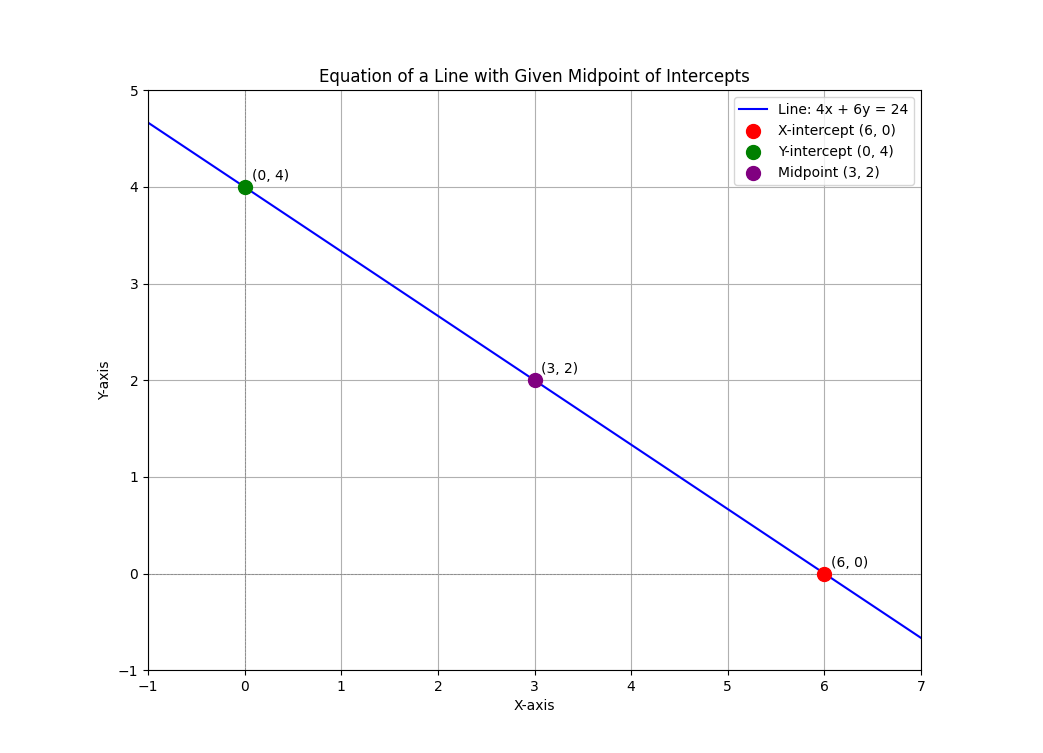
\includegraphics[width=0.9\columnwidth]{../figs/fig1.png}
\caption{}
\label{fig:1}
\end{figure}
\end{frame}

\begin{frame}{Plot by Python only}
\begin{figure}[H]
\centering
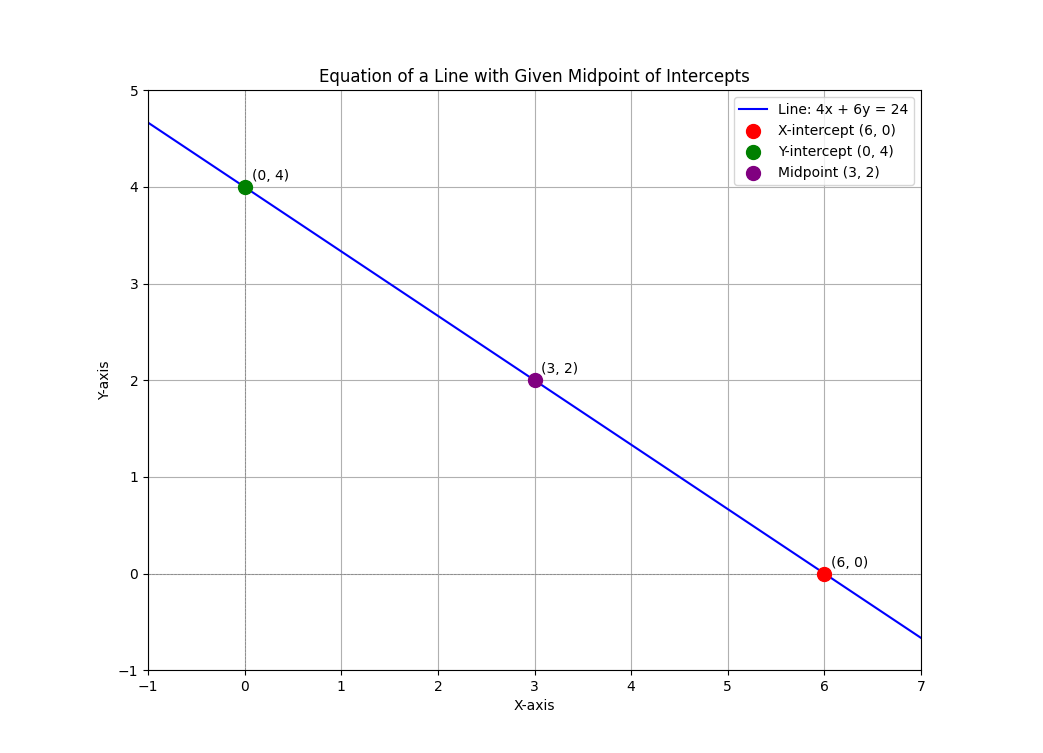
\includegraphics[width=0.9\columnwidth]{../figs/fig2.png}
\caption{}
\label{fig:2}
\end{figure}
\end{frame}

\end{document}
